%!TeX root=MemoriaTFG.tex

\chapter{Instruccions generals i itinerari del Treball Final de Grau }\label{instruccions}
\begin{figure}
\centering
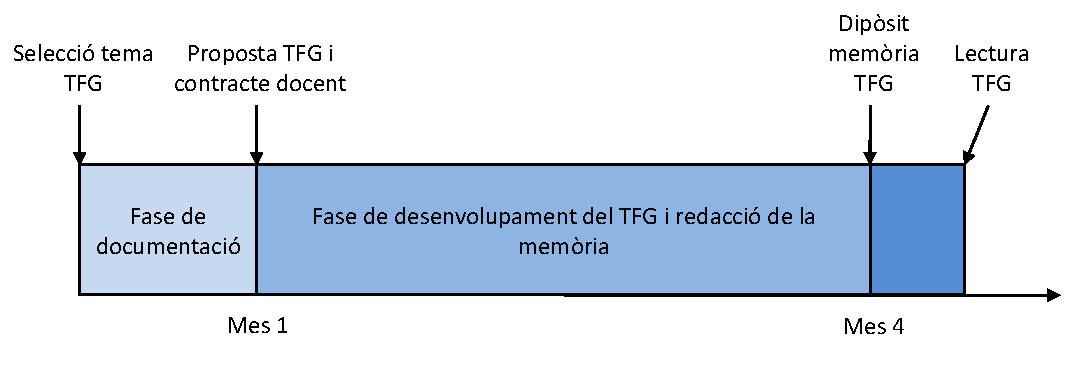
\includegraphics[width=\linewidth]{Itinerari_TFG}
\caption{\label{fig:itinerari}Itinerari del Treball Final de Grau}
\end{figure}

\section{Inici del Treball Final de Grau}

Com a norma general, tal com apareix reflectit en els plans d'estudis de gairebé totes les titulacions de grau, el \ac{TFG} s'hauria de realitzar en el segon semestre de quart curs. Tanmateix, tot i que aquestes s'agrupen en cursos i semestres, els estudis universitaris s'estructuren en assignatures. Així doncs, atesa la naturalesa integradora del \ac{TFG}, la recomanació general seria que abans de començar a realitzar el \ac{TFG} haguéssim aprovat la major part de les assignatures troncals i obligatòries del grau. De fet, l'ideal seria que només ens manquessin les assignatures que en el pla d'estudis corresponent es cursen simultàniament amb el \ac{TFG}.

\section{Selecció del tema de Treball Final de Grau}

Una de les vies més habituals per escollir el tema de \ac{TFG} és a través de l'apartat corresponent de la web de l'\acf{EPS}. En aquest cas, després de revisar les propostes realitzades pels diferents professors o grups de recerca involucrats en la docència de l'\ac{EPS}, escollirem les que més ens interessin i contactarem amb els professors responsables. Si algun dels professors encara no té el tema assignat i ens accepta, començarem a treballar en la fase de documentació i en la preparació de la proposta.

Existeixen altres possibilitats a l'hora d'escollir un tema de \ac{TFG}. Per exemple, podem realitzar el \ac{TFG} en una empresa del sector. En aquest cas és important que contactem amb un professor de l'\ac{EPS} que vulgui realitzar les tasques de supervisió i que pertanyi a un àrea de coneixement propera als continguts a tractar en el \ac{TFG}, d'aquesta manera ens assegurarem que la proposta de \ac{TFG} i el camp que aquesta cobreix compleixen amb els estàndards habituals a la nostra titulació. En cas de dubte, el més convenient és contactar amb el cap d'estudis de la titulació corresponent que segur que ens orientarà i ens proporcionarà la informació necessària.

Val a dir que el \ac{TFG} també es pot realitzar en una universitat amb la que s'hagin establert convenis de convalidació (programes Sèneca, Erasmus, Averroes, \ldots). Tanmateix, en aquest cas haurem de seguir els procediments administratius establerts en aquesta altra universitat.

\section{Preparació de la proposta i contracte docent}

Un cop escollit el tema de \ac{TFG} començarem a treballar en la fase de documentació i, d'acord amb el nostre supervisor, prepararem la proposta de \ac{TFG}. Per a la redacció d'aquesta proposta convé seguir les indicacions descrites al capítol \ref{proposta} i és recomanable que aquesta fase de documentació i preparació de la proposta de \ac{TFG}, tal com es mostra a la Fig. \ref{fig:itinerari}, no s'allargui més enllà d'un mes. Sobre la proposta de \ac{TFG} és sobre la que estudiant i professor signaran el contracte docent. En aquest contracte s'establiran els compromisos del professor quant a seguiment i supervisió del projecte i els de l'estudiant quant a dedicació i termini de presentació. La proposta de \ac{TFG} i el contracte docent, signat tant per l'alumne com pel professor, seran lliurats als serveis administratius on l'\ac{EPS} signarà el compromís de disponibilitat de medis materials genèrics i de formalització d'un tribunal de \ac{TFG} adient.

\section{Desenvolupament del Treball Final de Grau}

Un cop aprovada la proposta de \ac{TFG} ens dedicarem a la realització del \ac{TFG} i a la redacció de la memòria sota la supervisió del director i seguint les condicions estipulades en el contracte docent. Per a la redacció de la memòria convé seguir les indicacions descrites al capítol \ref{memoria}. És recomanable que aquesta fase de desenvolupament i redacció del treball, tal com ens mostra la Fig. \ref{fig:itinerari}, no superi els quatre mesos.

\section{Dipòsit de la memòria}

Una vegada acabada la seva redacció, i amb el vist-i-plau del nostre supervisor, dipositarem la memòria del \ac{TFG} a secretaria seguint les indicacions de la normativa de \acsp{TFG} de l'\ac{EPS}.

\section{Preparació de la presentació}

Finalment només ens quedarà preparar la presentació del \ac{TFG} per tal de fer-ne la defensa oral davant el tribunal. Per a la preparació d'aquesta presentació convé seguir les indicacions del capítol \ref{presentació}.
